Código para la toma de tiempos:

\begin{lstlisting}

float E_ABS = 0.01;
float E_REL = 0.001;
cronometro c;
    long int r = 0;
    c.activar();
    do {	
		List<Defense*>::iterator currentDefense = defenses.begin();
		while(currentDefense != defenses.end()) {
			// CÓDIGO RELEVANTE
            currentDefense++;
		}
		r++;
    } while(c.tiempo() < E_ABS/E_REL+E_ABS);
    c.parar();

\end{lstlisting}

Para la realización de la gráfica, primero ejecutamos la orden \textit{make data} para obtener los datos necesarios para la realización de la misma.
Luego ejecutamos la orden \textit{make plot} para que se genere la gráfica. (En mi caso no he hecho uso de esta instrucción, puesto que la he generado manualmente con los datos incluidos en 3 archivos diferentes. La orden que he usado ha sido \textit{plot "tiemposFusion.txt" w l, "tiemposRapida.txt" w l, "tiemposMonticulo.txt" w l})


\begin{lstlisting}

tiemposFusion.txt
16	1.01452e-05
196	0.000481283
576	0.0023466
1156	0.00862705
1936	0.0210874
2916	0.046946
2916	0.0582231
5476	0.158967
7056	0.256737
8836	0.401194
10816	0.59608

tiemposRapida.txt
16	1.05001e-05
196	0.000475255
576	0.00232522
1156	0.00924325
1936	0.0210499
2916	0.0477055
2916	0.0592517
5476	0.162935
7056	0.262465
8836	0.406422
10816	0.602452

tiemposMonticulo.txt
16	7.32998e-06
196	0.000460873
576	0.00234099
1156	0.00930774
1936	0.0218267
2916	0.0515109
2916	0.0618922
5476	0.16398
7056	0.258604
8836	0.412018
10816	0.596913

\end{lstlisting}

\begin{figure}
\centering
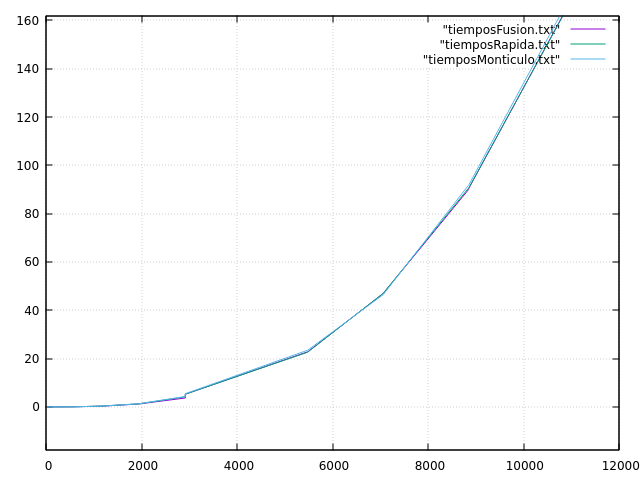
\includegraphics[width=0.7\linewidth]{./grafica}
\caption{Tiempos}
\label{fig:grafica}
\end{figure}
